\documentclass[12pt]{article}
%\usepackage[english]{babel}
\RequirePackage[spanish]{babel}
\usepackage[spanish]{babel}
\usepackage{graphicx}
%\usepackage[pdftex,bookmarks,colorlinks,breaklinks]{hyperref}  % PDF hyperlinks, with coloured links
\usepackage[pdftex,bookmarks,breaklinks]{hyperref}  % PDF hyperlinks, with coloured links
\usepackage[utf8]{inputenc}
\usepackage{epstopdf}
\usepackage{fullpage}
\usepackage{url}
\usepackage{lscape}
\usepackage{float}
\renewcommand{\baselinestretch}{1.5}
\usepackage{caption}
\usepackage{wrapfig}
\usepackage[official]{eurosym}
\parskip 3ex % espacio entre parrafos.
\makeatletter
\renewcommand\paragraph{\@startsection{paragraph}{4}{\z@}%
	{-2.5ex\@plus -1ex \@minus -.25ex}%
	{1.25ex \@plus .25ex}%
	{\normalfont\normalsize\bfseries}}
\makeatother
\setcounter{secnumdepth}{4} % how many sectioning levels to assign numbers to
\setcounter{tocdepth}{4}    % how many sectioning levels to show in ToC


\begin{document}

%%%%%%%%%%%%%%% PORTADA UDG %%%%%%%%%%%%%%%%%%
\pagestyle{empty}
\begin{tabular}{|p{\textwidth}|}
    \hline
    \vspace{.5mm}
    
\includegraphics[scale=.7]{imgs/udg.png}\\
    \bigskip
    \begin{center}
        \begin{Huge} \textbf{Treball final de grau} \end{Huge}
    \end{center}\\
    \hline
    \vspace{1mm}
    \begin{large} \textbf{Estudi: Grau en Disseny i Desenvolupament de Videojocs} \end{large}
    \vspace{5mm}\\
    \hline
    \vspace{1mm}
    \begin{large} \textbf{Títol: La Influencia de los Videojuegos en Nuestra Moral} \end{large}
    \vspace{5mm}\\
    \hline
    \vspace{1mm}
    \begin{large} \textbf{Document: Resumen} \end{large}
    \vspace{5mm}\\
    \hline
    \vspace{1mm}
    \begin{large} \textbf{Alumne: José Francisco Riffo Astete} \end{large}
    \vspace{5mm}\\
    \hline
    \vspace{1mm}
    \begin{large} \textbf{Tutor: Imma Boada Oliveras} \end{large}\\
    \begin{large} \textbf{Departament: IMAE} \end{large}\\
    \begin{large} \textbf{Àrea: LSI} \end{large}\\[5mm]
    \hline
    \vspace{1mm}
    \begin{large} \textbf{Convocatòria (mes/any): Setembre 2020} \end{large}
    \vspace{5mm}\\
    \hline
\end{tabular}

%%%%%%%%%%%%%%%%%%%%%%%%%%%%%%%%%%%%%%%
\newpage
\pagestyle{plain}

\section{Introducción}
Desde el inicio de los videojuegos es habitual que el jugador deba enfrentarse a la toma de decisiones, desde los juegos más sencillos como Tetris -donde debes decidir donde colocar la siguiente pieza- hasta juegos más complejos como Detroit: Become Human, en el cual cada acción que realizas y cada dialogo que escoges tiene un impacto en la historia.

\begin{figure}[h]
    \centering
    \begin{minipage}{.3\textwidth}
        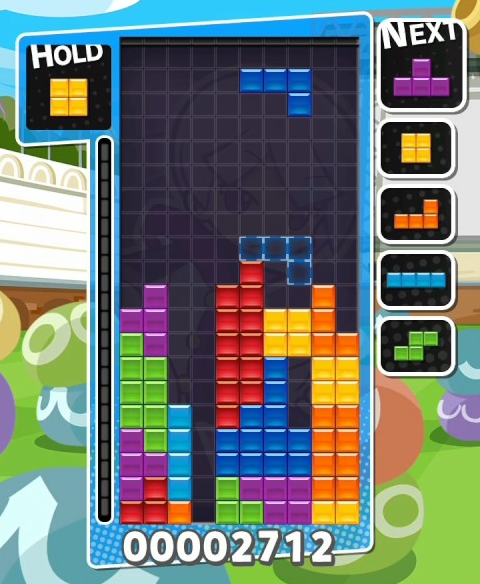
\includegraphics[width=\textwidth]{imgs/tetris.png}
        \caption*{Tetris}
    \end{minipage}
    \begin{minipage}{.69\textwidth}
        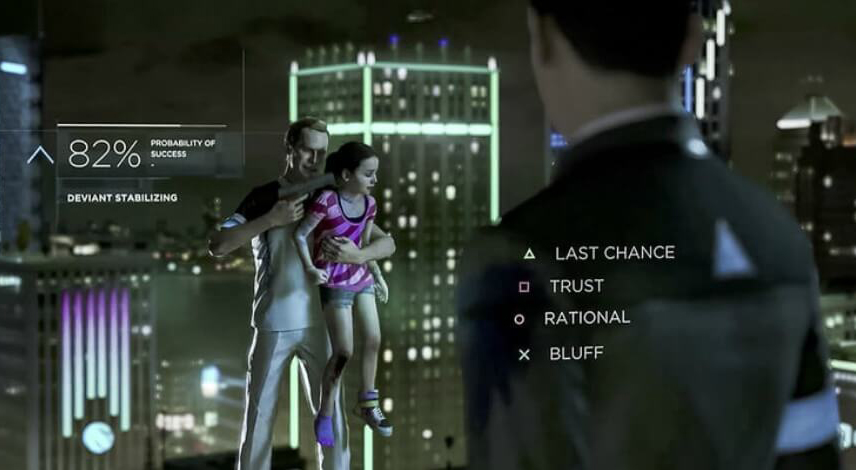
\includegraphics[width=\textwidth]{imgs/detroit-choices.jpg}
        \caption*{Detroit: Become Human}
    \end{minipage}
\end{figure}

Este proyecto busca investigar aquellas decisiones desde el punto de vista de un dilema moral, y más precisamente, saber si estos dilemas son significativos para el jugador y pueden cambiar su moral.

\subsection{Objetivo}
El objetivo de este proyecto es evaluar experimentalmente el impacto que los videojuegos y sus dilemas morales pueden tener sobre las personas.

Para alcanzar este objetivo se deberá:
\begin{itemize}
    \item Diseñar e implementar un videojuego en el que la toma de decisiones juegue un papel fundamental. Nos interesará que estas decisiones queden integradas en la historia del juego. Se le presentará un dilema moral inicial al jugador, y dependiendo de su respuesta, el videojuego y su historia trataran de influenciar al jugador para que cambie su opción.
    \item Diseñar y realizar un estudio con cuestionarios pre- y post- juego que nos permita analizar el comportamiento del jugador.
    \item Analizar los datos obtenidos en las sesiones de prueba para comprobar la hipótesis planteada y ver como el videojuego afectó a los jugadores.
\end{itemize}

\section{Diseño del Videojuego}
Para alcanzar el primer objetivo se diseño e implementó un videojuego en donde la toma de decisiones juega un papel fundamental, y en el cual la historia tratar de influenciar al jugador para hacerlo cambiar de decisión. Adicionalmente se realizó un estudio con cuestionarios pre- y post- juego que permitieron analizar el comportamiento del jugador y su moral, para ser precisos se utilizó el “Moral Foundations Questionnaire”.

\subsection{Narrativa}
En el juego sigues la historia de Lucía, una chica universitaria de 20 años de edad que está abrumada por la presión que sus padres y la universidad le exigen. Se tocan los temas de la depresión y el suicidio, y es que la vida de esta chica está en manos del jugador tanto al inicio como al final del videojuego.

\begin{wrapfigure}{r}{5cm}
    \centering
    
\includegraphics{imgs/lucia.png}
    \caption*{Lucía}
\end{wrapfigure}

Si el jugador deja vivir a Lucía al inicio, la acompaña en un día donde tiene un examen importante en su universidad, donde el estrés, la soledad, y la angustia son componentes que la acompañan todo el tiempo. El juego intentará hacer que el jugador elija que Lucía muera al final.

Si el jugador deja morir a Lucía al inicio, aparece La Muerte en el juego, un ente neutral que muestra a Lucía las razones por las que ha muerto, pero también le muestra que su vida no era tan mala. Se repasan una serie de recuerdos y memorias de Lucía que ella creía ya olvidados. El juego intentará hacer que el jugador elija que Lucía viva al final.

\subsection{Mecánicas}
El juego implementa 6 distintos minijuegos (3 por cada ruta) los cuales buscan transmitir las emociones de Lucía al jugador. Apoyan la narrativa y buscan hacer que el jugador cambie de opción al final del juego.

\begin{figure}[h]
    \centering
    \begin{minipage}{.15\textwidth}
        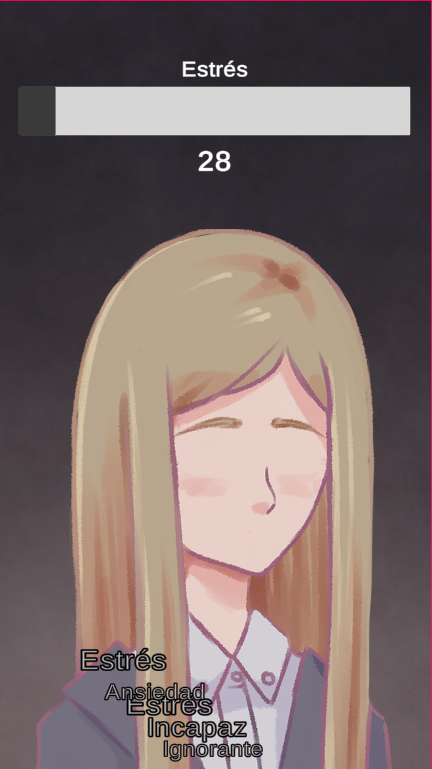
\includegraphics[width=\textwidth]{imgs/screenshot3.png}
    \end{minipage}
    \begin{minipage}{.15\textwidth}
        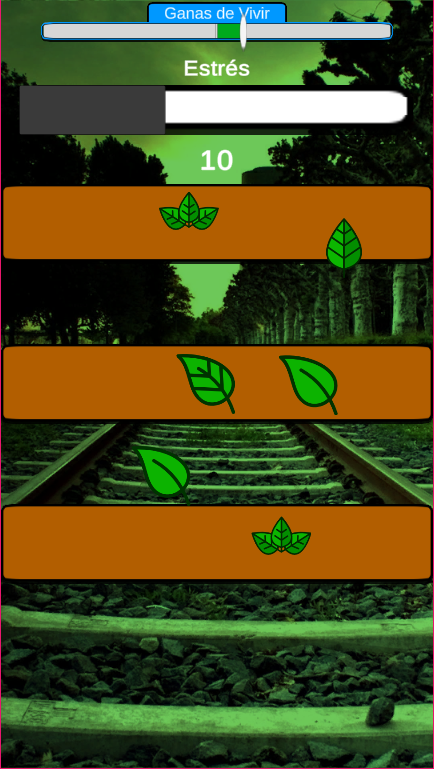
\includegraphics[width=\textwidth]{imgs/screenshot12.png}
    \end{minipage}
    \begin{minipage}{.15\textwidth}
        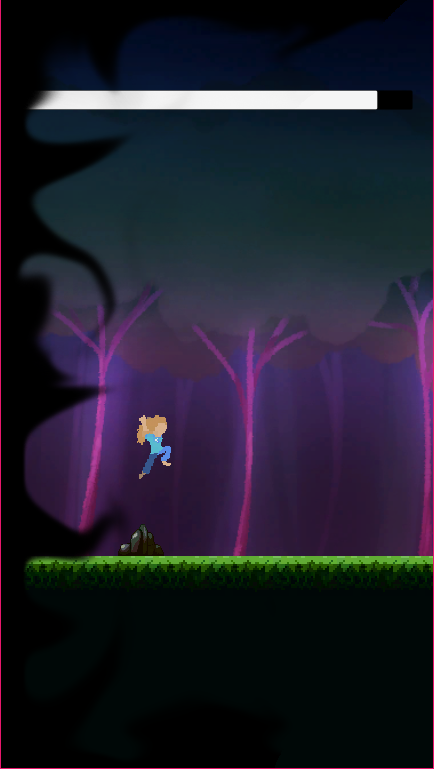
\includegraphics[width=\textwidth]{imgs/screenshot6.png}
    \end{minipage}
    \begin{minipage}{.15\textwidth}
        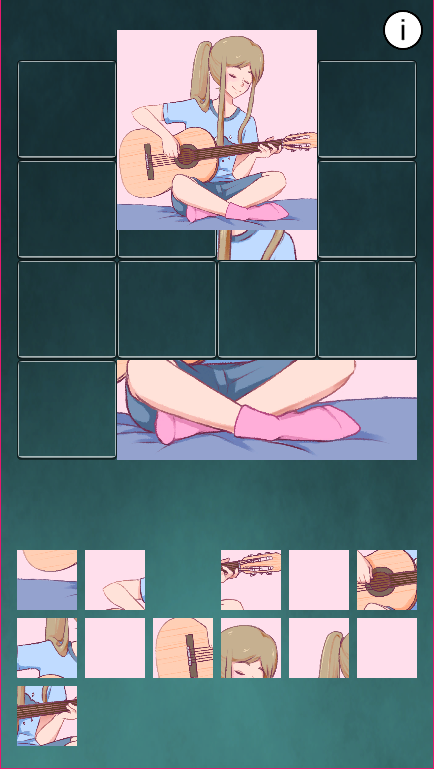
\includegraphics[width=\textwidth]{imgs/screenshot8.png}
    \end{minipage}
    \begin{minipage}{.15\textwidth}
        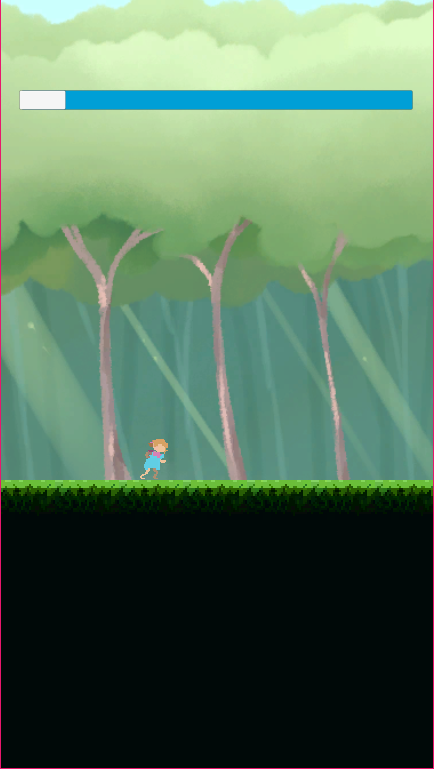
\includegraphics[width=\textwidth]{imgs/screenshot9.png}
    \end{minipage}
    \begin{minipage}{.15\textwidth}
        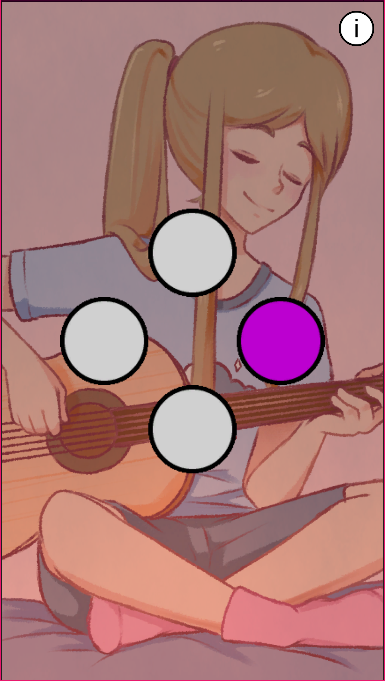
\includegraphics[width=\textwidth]{imgs/screenshot14.png}
    \end{minipage}
    \caption*{Minijuegos implementados}
\end{figure}

\section{Resultados}
El videojuego fue implementado utilizando el motor Unity3D, y obtuvo una buena recepción por parte de los jugadores, quienes dieron opiniones positivas al respecto.
Se consiguieron datos de 48 personas distintas que jugaron al juego. Se compararon las distintas decisiones que tomaron estos usuarios y se contrastaron los datos de el cuestionario de moralidad, para ver si el juego había logrado influir en los usuarios o si no los afectó en lo absoluto.

\begin{figure}[h]
    \centering
    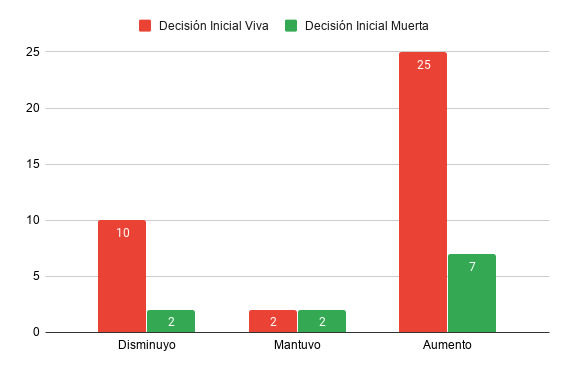
\includegraphics[scale=.7]{imgs/resultado-encuesta-separado.png}
    \caption*{Variación en el resultado del cuestionario}
\end{figure}

\begin{figure}[h]
    \centering
    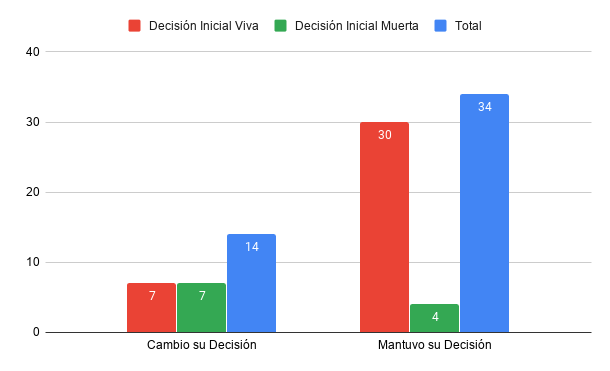
\includegraphics[scale=.7]{imgs/resultado-decision.png}
    \caption*{Cantidad de jugadores que cambiaron o mantuvieron su decisión inicial}
\end{figure}

Los datos del cuestionario realizado muestran que el juego si influyó en la moral de los usuarios, principalmente en el área asociadas a los sistemas de empatía y apego que sienten las personas por otras, no obstante, esta influencia fue leve ya que la mayoría mantuvo la decisión que eligió al comienzo del videojuego.

\section{Conclusiones}
Esta leve influencia puede deberse a lo corto del juego (La sesión de juego es inferior a los 10 minutos) en donde la narrativa no acaba de desarrollarse o profundizar completamente.

Un estudio con un juego más largo en donde los usuarios estén más expuestos al dilema podría otorgar datos que muestren una influencia mayor, sin embargo aquello es criterio para otra investigación.

Aún así, los datos concluyen que los usuarios si fueron -en mayor o menor medida- influidos por el videojuego, dando por cierta la hipótesis inicial que se prentendia investigar.

\end{document}